\section{Gallery-Level Alignment}
\label{sec:method}

\begin{figure}[t]
  \centering
  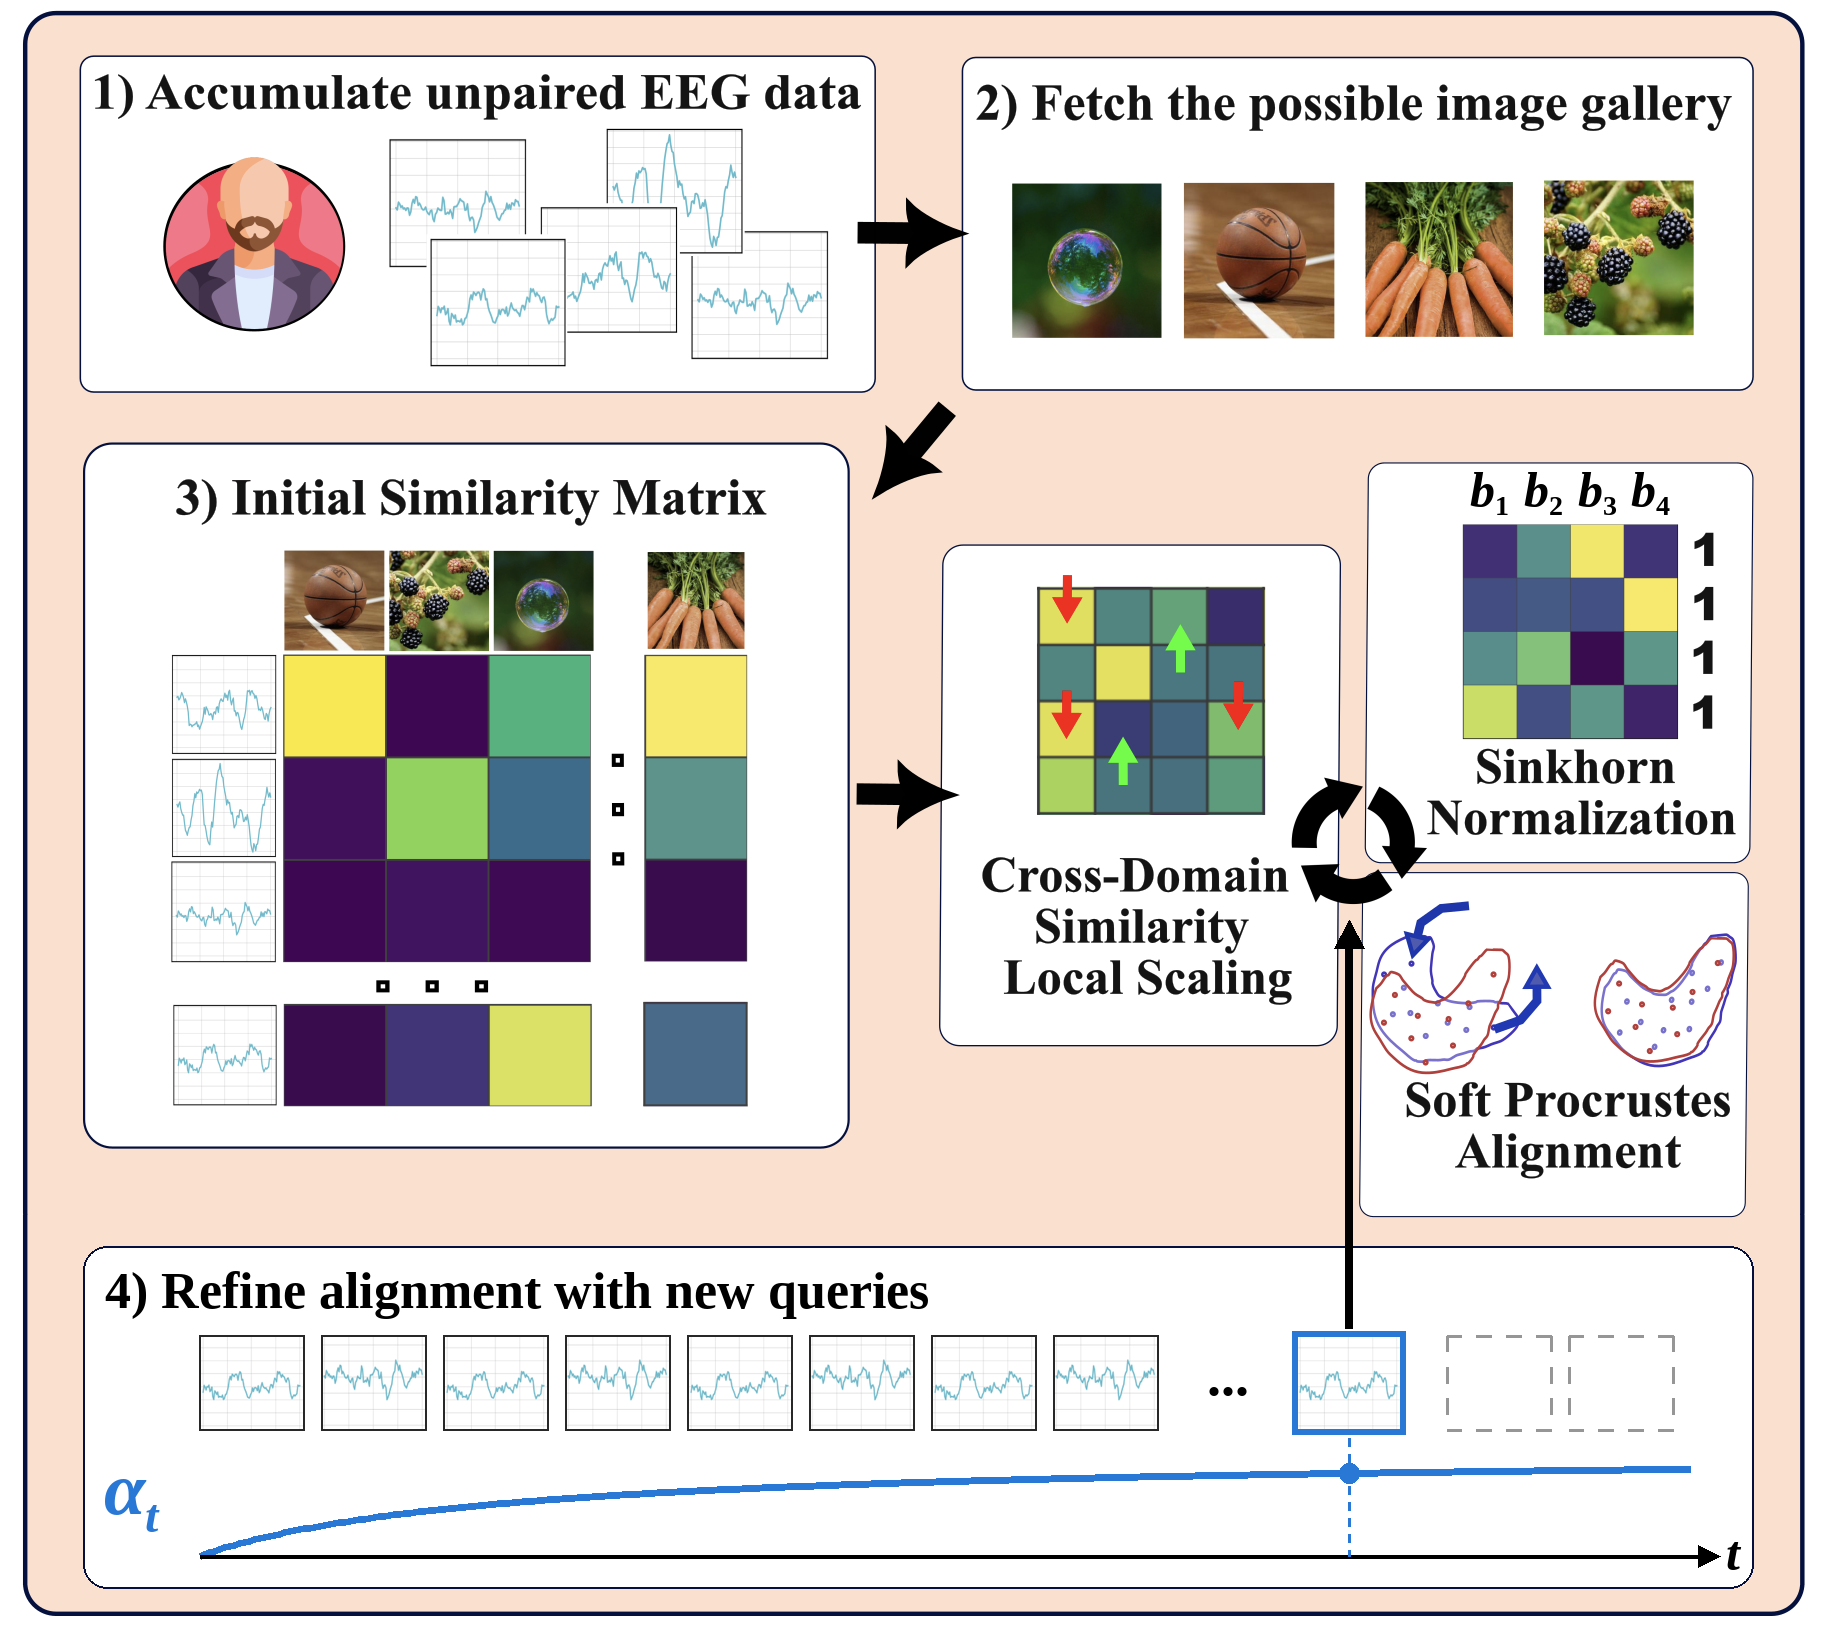
\includegraphics[width=\columnwidth]{figures/GALA_v2.png}
  \caption{GALA. The unlabeled EEG embeddings of an unseen subject are whitened, compared with the gallery through cross-domain similarity local scaling, and registered onto it by a Sinkhorn normalization with estimated column masses $b_j$ and a soft Procrustes alignment. Each new query (blue) triggers one pass of this loop.}
  \label{fig:pipeline}
\end{figure}


At step $t$ of a session, the decoder holds the buffer  
 $\Em = [\ev_1^\top,\ldots,\ev_N^\top]^\top \in \R^{N\times d}$ of all the EEG embeddings received so far, with $N=t$, and the gallery $\Vm = [\vv_1^\top,\ldots,\vv_K^\top]^\top \in \R^{K\times d}$, the embedding of the $K$ candidate images, which are known in advance (A1). The gallery is fixed and does not depend on the user, whereas the buffer grows during the session, and the correspondence between queries and gallery images is unknown. GALA registers the buffer onto the gallery.  
\subsection{A prior for incremental calibration}
\label{sec:prior}
In the incremental setting, the calibration is updated after every query (A2), including at the start of a session, when the
buffer holds only a few queries in a $d$-dimensional space. Every quantity
estimated from the buffer is then unreliable, and a calibration that trusts
the buffer fully risks making the decoder worse than no calibration.
GALA is therefore built on one principle: the zero-shot decoder is a prior
worth $n_0$ observations, and the whitening and the rotation estimated from the
buffer are combined with their zero-shot values, with a weight on the buffer of
%
\begin{equation}
  \alpha_t = \frac{t}{t + n_0}.
  \label{eq:alpha}
\end{equation}
%
This prior enters the registration below: the moments used
for whitening shrink towards those of an isotropic cloud centered at the
origin, and the rotation is pulled towards the identity.
At $t = 0$, the whitening and the rotation are the identity, and GALA decodes
the zero-shot embeddings; as $t$ grows, the weight of
the prior vanishes and GALA converges to the unregularized registration.

\subsection{Whitening and registration}
\label{sec:problem}


As discussed in Sec.~\ref{sec:setting}, the buffer behaves as a distorted copy of the queried
part of the gallery. We model this distortion as a translation and an
anisotropic scaling, which whitening removes, followed by a change of
orientation, which the registration estimates jointly with the unknown
correspondences.
\paragraph{Whitening.}
Let $\muv$ and $\Sigmam$ be the mean and covariance of the buffer,
\begin{equation} \label{eq:moments}
\muv = \frac{1}{N}\sum_{i=1}^{N} \ev_i,
\qquad
\Sigmam = \frac{1}{N}\sum_{i=1}^{N}(\ev_i-\muv)(\ev_i-\muv)^\top .
\end{equation}
Following the prior of Sec.~\ref{sec:prior}, the mean is shrunk towards the origin and the covariance towards an isotropic one,
\begin{equation} \label{eq:shrunk}
\widetilde{\muv} = \alpha_t\,\muv,
\qquad
\widetilde{\Sigmam} = \alpha_t(1-\rho)\,\Sigmam + \big(1-\alpha_t(1-\rho)\big)\,\frac{\operatorname{tr}(\Sigmam)}{d}\, \I_d ,
\end{equation}
where $\rho$ is a shrinkage coefficient~\cite{ledoit2004honey}. The whitened and normalized EEG embeddings are
\begin{equation}\label{eq:whitening}
\widetilde{\ev}_i = \frac{\widetilde{\Sigmam}^{-1/2}(\ev_i-\widetilde{\muv})}{\|\widetilde{\Sigmam}^{-1/2}(\ev_i-\widetilde{\muv})\|}.
\end{equation}
We denote by $\widetilde{\Em}$ the matrix whose rows are $\widetilde{\ev}_i$. This step is the embedding-space counterpart of re-centering in classical BCI~\cite{zanini2018transfer,he2020euclidean}.
\paragraph{Registration problem.}
We estimate an orthogonal map $\mathbf{R}$, the query frequencies
$\mathbf{b}$ of the gallery images in the probability simplex $\Delta_K$, and a soft correspondence matrix
$\mathbf{P} \in \R_+^{t\times K}$ between queries and gallery images, by solving
%
\begin{subequations}\label{eq:problem}
    \begin{equation}
         \max_{\substack{\mathbf{R}^\top\mathbf{R} = \I_d,\ \mathbf{b} \in \Delta_K \\ \mathbf{P} \in \Pi(\mathbf{a},\mathbf{b})}}\;
   \big\langle \mathbf{P}, \mathbf{S}(\mathbf{R}) \big\rangle
  + \tau_{\mathrm{sk}}\, H(\mathbf{P})
  - \frac{n_0\,\bar\sigma}{2t}\,\big\|\mathbf{R} - \I_d\big\|^2 \label{eq:problema}
   \end{equation}
   \begin{equation}
         \text{s.t.}\quad  \mathbf{b} \in \arg\max_{\mathbf{b} \in \Delta_K}\, \ell(\mathbf{b}; \mathbf{R}),\label{eq:freq}
    \end{equation}
   \end{subequations} 
%
where $S_{ij}(\mathbf{R}) = \cos(\widetilde{\ev}_i\mathbf{R}, \vv_j)$ is the
similarity after registration, $H(\mathbf{P}) = -\sum_{ij}P_{ij}(\log P_{ij}-1)$
is the entropy of the correspondences, whose softness is controlled by the
temperature $\tau_{\mathrm{sk}}$, and
%
\begin{equation}
  \Pi(\mathbf{a},\mathbf{b}) = \big\{\mathbf{P} \ge 0 \,:\,
  \mathbf{P}\mathbf{1}_K = \mathbf{a},\ \mathbf{P}^\top\mathbf{1}_t = \mathbf{b}\big\}
  \label{eq:polytope}
\end{equation}
%
is the set of plans in which each query carries the mass
$\mathbf{a} = \tfrac1t\mathbf{1}_t$ and gallery image $j$ receives the mass
$b_j$. The last term is the prior of
Sec.~\ref{sec:prior} on the rotation; $\bar\sigma$, the mean singular value of
$\widetilde{\Em}^\top\mathbf{P}\Vm$, sets its scale. 

The masses $\mathbf{b}$ are the query frequencies, and estimating them lets GALA account for assumptions (A3) and (A4) of the incremental transductive calibration setting. GALA
therefore treats $\mathbf{b}$ as a variable, estimated from the buffer through the
constraint of~\eqref{eq:problem}. Each query is assigned to the gallery
independently of the others,
$\pi_{ij}(\mathbf{R}) = \exp(S_{ij}(\mathbf{R})/\tau_{\mathrm{sk}}) / \sum_{l}\exp(S_{il}(\mathbf{R})/\tau_{\mathrm{sk}})$,
and $\ell$ is the log-likelihood of these soft assignments under the
frequencies $\mathbf{b}$, with a symmetric Dirichlet prior worth $n_b$ queries per
image,
\begin{equation*}
  \ell(\mathbf{b};\mathbf{R}) =
  \sum_{j=1}^{K}\left(\sum_{i=1}^{t}\pi_{ij}
  \;+\; n_b \right)\log b_j
  \;=\; \sum_{j=1}^{K} w_j \log b_j.
\end{equation*}
Since all vectors have unit norm and $\mathbf{R}$ is orthogonal,
$\langle \mathbf{P}, \mathbf{S}(\mathbf{R})\rangle = \operatorname{tr}(\mathbf{R}^\top\widetilde{\Em}^\top\mathbf{P}\Vm)
= 1 - \tfrac12\sum_{i,j}P_{ij}\|\widetilde{\ev}_i\mathbf{R} - \vv_j\|^2$, so that without the prior term,
problem~\eqref{eq:problem} is the entropic Wasserstein--Procrustes problem~\cite{grave2019wasserstein}, which
minimizes the transport cost between the two clouds.

% ------------------------------------------------------------
% placed here (source on page 5) so that it appears at the top of page 6
\begin{figure*}[t]
  \centering
  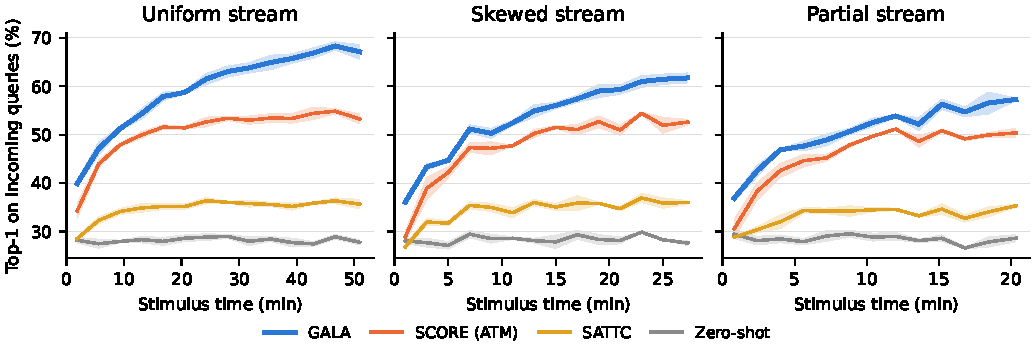
\includegraphics[width=\textwidth]{figures/final_incremental.pdf}
  \caption{Incremental transductive calibration on THINGS-EEG-2 (10 subjects, $q=20$). Top-1 accuracy of the incoming queries, each decoded before it is used for calibration, in windows of one fifteenth of the stream, against stimulus time, for the uniform, skewed and partial streams (mean $\pm$ one standard deviation over three training seeds). The figure shows four methods, all with the ATM encoder; Table~\ref{tab:inc} reports every method.}
  \label{fig:inc}
\end{figure*}

\subsection{Incremental update}
\label{sec:algo}

For fixed frequencies $\mathbf{b}$, problem~\eqref{eq:problem} is not jointly concave, but each block has an exact solution when the other is fixed, and we
solve it by alternating maximization. After
each query, GALA performs a single pass, starting from the rotation of the
previous step: it first updates the frequencies $\mathbf{b}$, then the
correspondences and the rotation (Alg.~\ref{alg:gala}).
\begin{algorithm}[ht!]
\caption{Update of GALA after query $t$.}
\label{alg:gala}
\begin{algorithmic}[1]
\Require buffer $\Em \in \R^{t\times d}$, gallery $\Vm \in \R^{K\times d}$, previous rotation $\mathbf{R}_{t-1}$ ($\mathbf{R}_0 = \mathbf{I}_d$);
         $n_0$, $n_b$, $\rho$, $\tau_{\mathrm{sk}}$, $\gamma$, $k$, $\mathbf{a}$
\State $\alpha_t \gets t/(t+n_0)$
\State $\widetilde{\Em} \gets$ whitened and normalized queries, Eqs.~\eqref{eq:moments}--\eqref{eq:whitening}
\State $\widehat{\mathbf{S}} \gets$ CSLS scores of $\widetilde{\Em}\mathbf{R}_{t-1}$ and $\Vm$, Eq.~\eqref{eq:csls}
\State $\mathbf{b} \gets$ estimated query frequencies, Eq.~\eqref{eq:masses}
\State $\mathbf{P} \gets \operatorname{Sinkhorn}\big(\exp(\widehat{\mathbf{S}}/\tau_{\mathrm{sk}});\,\mathbf{a},\mathbf{b}\big)$
\State $\mathbf{R}_t \gets \mathbf{U}\mathbf{W}^\top$, with $\mathbf{U}\mathbf{D}\mathbf{W}^\top$ the SVD of $\mathbf{M}$ in Eq.~\eqref{eq:M}, using $\mathbf{P}^{\circ\gamma}$
\State \Return the whitening and $\mathbf{R}_t$: query $t+1$ is decoded by $\arg\max_j$ of its CSLS scores after whitening and rotation
\end{algorithmic}
\end{algorithm}

\paragraph{Query frequencies.} For fixed $\mathbf{R}$, the frequencies are estimated
from the buffer. Maximizing~\eqref{eq:freq} under the constraint
$\sum_j b_j = 1$, with a Lagrange multiplier, gives $b_j = w_j / \sum_l w_l$. Since each row of $\boldsymbol{\pi}$
sums to one, $\sum_l w_l = K n_b + t$, and the mass of image $j$ is its soft
number of queries, combined with the prior of $n_b$ queries per image:
%
\begin{equation}
  b_j = \frac{n_b + \sum_{i=1}^{t}\pi_{ij}}{K n_b + t}.
  \label{eq:masses}
\end{equation}
%
At the start of a session, the masses are thus uniform, and they follow the
frequencies observed in the buffer as it grows.

\paragraph{Correspondence step.} For fixed $\mathbf{R}$ and $\mathbf{b}$, the optimal plan is
$\mathbf{P} = \operatorname{diag}(\mathbf{f})\exp(\mathbf{S}/\tau_{\mathrm{sk}})\operatorname{diag}(\mathbf{g})$,
where the scaling vectors $\mathbf{f} \in \R_+^N$ and $\mathbf{g} \in \R_+^K$ are computed by Sinkhorn
iterations~\cite{sinkhorn1964,cuturi2013sinkhorn} so that
$\mathbf{P} \in \Pi(\mathbf{a},\mathbf{b})$.

\paragraph{Rotation step.} For fixed $\mathbf{P}$, using the trace form of the alignment term and
$\|\mathbf{R}-\mathbf{I}_d\|_F^2 = 2d - 2\operatorname{tr}(\mathbf{R})$ for an orthogonal
$\mathbf{R}$, problem~\eqref{eq:problem} reduces to
$\max_{\mathbf{R}^\top\mathbf{R} = \mathbf{I}_d}\operatorname{tr}\big(\mathbf{R}^\top\mathbf{M}\big)$ with
%
\begin{equation}
  \mathbf{M} = \widetilde{\Em}^\top\mathbf{P}\,\Vm + \frac{n_0}{t}\,\bar\sigma\,\mathbf{I}_d ,
  \label{eq:M}
\end{equation}
%
an orthogonal Procrustes problem whose solution is $\mathbf{R} = \mathbf{U}\mathbf{W}^\top$,
where $\mathbf{U}\mathbf{D}\mathbf{W}^\top$ is the singular value decomposition of
$\mathbf{M}$~\cite{schonemann1966procrustes}. The prior term only adds
$\tfrac{n_0}{t}\bar\sigma\,\mathbf{I}_d$ to the data matrix: in directions where
the buffer carries little evidence, $\mathbf{M}$ is dominated by this term and
$\mathbf{R}$ stays close to the identity.

\paragraph{Practical choices.}
GALA departs from the exact block updates in two ways, both validated in Sec.~\ref{sec:ablation}.
First, since nearest-neighbour retrieval in high dimension is biased towards
hub images~\cite{radovanovic2010hubs}, the similarity $\mathbf{S}$ is replaced by the
Cross-domain Similarity Local Scaling score~\cite{conneau2018muse},
%
\begin{equation}
  \widehat{S}_{ij} = 2\cos(\widetilde{\ev}_i\mathbf{R}, \vv_j)
  - r_V(\widetilde{\ev}_i\mathbf{R}) - r_E(\vv_j),
  \label{eq:csls}
\end{equation}
%
where $r_V(\mathbf{x})$ is the mean cosine similarity of a query $\mathbf{x}$ to
its $k$ nearest gallery images, and $r_E(\vv_j)$ that of image $\vv_j$ to its $k$
nearest queries of the buffer. Second, the rotation step uses the sharpened plan
$\mathbf{P}^{\circ\gamma}$ in~\eqref{eq:M} and in $\bar\sigma$, the element-wise power with
$\gamma \ge 1$, which gives more weight to confident correspondences, and the
gallery embeddings in $\mathbf{M}$ are not normalized. An
incoming query is whitened, rotated and decoded with its CSLS scores,
$\hat\jmath = \arg\max_j \widehat{S}_{ij}$ (Alg.~\ref{alg:gala}).
